\documentclass[border=8pt, multi, tikz]{standalone} 
\usepackage{import}
\subimport{./layers/}{init}
\usetikzlibrary{positioning}
\usetikzlibrary{3d} %for including external image 


\def\ConvColor{rgb:yellow,5;red,2.5;white,5}
\def\ConvReluColor{rgb:yellow,5;red,5;white,5}
\def\PoolColor{rgb:red,1;black,0.3}
\def\UnpoolColor{rgb:blue,2;green,1;black,0.3}
\def\FcColor{rgb:blue,2;green,5;white,5}
\def\FcReluColor{rgb:blue,2;green,5;white,4}
\def\SoftmaxColor{rgb:magenta,5;black,7}   
\def\OutputColor{rgb:blue,1}


\newcommand{\copymidarrow}{\tikz \draw[-Stealth,line width=0.8mm,draw={rgb:blue,4;red,1;green,1;black,3}] (-0.3,0) -- ++(0.3,0);}

\begin{document}
\begin{tikzpicture}
\tikzstyle{connection}=[ultra thick,every node/.style={sloped,allow upside down},draw=\edgecolor,opacity=0.7]
\tikzstyle{copyconnection}=[ultra thick,every node/.style={sloped,allow upside down},draw={rgb:blue,4;red,1;green,1;black,3},opacity=0.7]

\node[canvas is zy plane at x=-0.3](temp) at (0,0,-8) {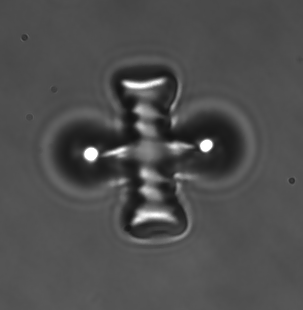
\includegraphics[width=-8.96cm,height=8.96cm]{images/input.png}};
    \node at (-2,-7.7,-2) {\textbf{\large{Input Image}}};
	\path (0,0,0);
\pic[shift={(0,0,0)}] at (0,0,0) 
    {Box={
        name=conv0,
        caption= ,
        xlabel={{3, }},
        ylabel=224,
        zlabel=\qquad 224,
        fill=\ConvColor,
        height=44.8,
        width=0.1,
        depth=44.8
        }
    };


\pic[shift={(1,0,0)}] at (conv0-east) 
    {Box={
        name=conv1,
        caption=\textbf{\large{Conv1}},
        xlabel={{96, }},
        ylabel=55,
        zlabel=55,
        fill=\ConvColor,
        height=11.0,
        width=4.8,
        depth=11.0
        }
    };


\draw [connection]  (conv0-east)    -- node {\midarrow} (conv1-west);


\pic[shift={ (0,0,0) }] at (conv1-east) 
    {Box={
        name=pool1,
        caption= ,
        fill=\PoolColor,
        opacity=0.5,
        height=5.4,
        width=1,
        depth=5.4
        }
    };


\pic[shift={(1,0,0)}] at (pool1-east) 
    {Box={
        name=conv2,
        caption= \textbf{\large{Conv2}},
        xlabel={{256, }},
        ylabel=27,
        zlabel=27,
        fill=\ConvColor,
        height=5.4,
        width=11,
        depth=5.4
        }
    };


\draw [connection]  (pool1-east)    -- node {\midarrow} (conv2-west);


\pic[shift={ (0,0,0) }] at (conv2-east) 
    {Box={
        name=pool2,
        caption= ,
        fill=\PoolColor,
        opacity=0.5,
        height=2.6,
        width=1,
        depth=2.6
        }
    };


\pic[shift={(1,0,0)}] at (pool2-east) 
    {Box={
        name=conv3,
        caption= \textbf{\large{Conv3}},
        xlabel={{384, }},
        ylabel=13,
        zlabel=13,
        fill=\ConvColor,
        height=2.6,
        width=17,
        depth=2.6
        }
    };


\draw [connection]  (pool2-east)    -- node {\midarrow} (conv3-west);


\pic[shift={(1,0,0)}] at (conv3-east) 
    {Box={
        name=conv4,
        caption= \textbf{\large{Conv4}},
        xlabel={{384, }},
        ylabel=13,
        zlabel=13,
        fill=\ConvColor,
        height=2.6,
        width=17,
        depth=2.6
        }
    };


\draw [connection]  (conv3-east)    -- node {\midarrow} (conv4-west);


\pic[shift={(1,0,0)}] at (conv4-east) 
    {Box={
        name=conv5,
        caption= \textbf{\large{Conv5}},
        xlabel={{256, }},
        ylabel=13,
        zlabel=13,
        fill=\ConvColor,
        height=2.6,
        width=11,
        depth=2.6
        }
    };


\draw [connection]  (conv4-east)    -- node {\midarrow} (conv5-west);


\pic[shift={ (0,0,0) }] at (conv5-east) 
    {Box={
        name=pool3,
        caption= ,
        fill=\PoolColor,
        opacity=0.5,
        height=1.2,
        width=1,
        depth=1.2
        }
    };


\pic[shift={(1,0,0)}] at (pool3-east) 
    {Box={
        name=Fc1,
        caption= \textbf{\large{FC1}},
        xlabel={{1, }},
        ylabel=1,
        zlabel=\qquad 4096,
        fill=\FcColor,
        height=1,
        width=1,
        depth=40.96
        }
    };


\draw [connection]  (pool3-east)    -- node {\midarrow} (Fc1-west);


\pic[shift={(1,0,0)}] at (Fc1-east) 
    {Box={
        name=Fc2,
        caption= \textbf{\large{FC2}},
        xlabel={{1, }},
        ylabel=1,
        zlabel=\qquad 4096,
        fill=\FcColor,
        height=1,
        width=1,
        depth=40.96
        }
    };


\draw [connection]  (Fc1-east)    -- node {\midarrow} (Fc2-west);


\pic[shift={(1,0,0)}] at (Fc2-east) 
    {Box={
        name=soft1,
        caption=\textbf{\large{FC3 (ReLu)}},
        xlabel={{" ","dummy"}},
        zlabel=\qquad 16,
        fill=\SoftmaxColor,
        opacity=0.8,
        height=1,
        width=1,
        depth=5
        }
    };


\draw [connection]  (Fc2-east)    -- node {\midarrow} (soft1-west);

\pic[shift={(1,0,0)}] at (soft1-east) {
	RightBandedBox={
		name=output,
		caption=\makebox[0pt]{
					 \shortstack[c]{Output}},
		xlabel={{"1",""}},
            ylabel=1,
		zlabel=1,
		fill=\OutputColor,
		height=1,
		width=1,
		depth=1
	    }
        };
\draw [connection]  (soft1-east)    -- node {\midarrow} (output-west);

\end{tikzpicture}
\end{document}